% Results
%
%	some important things to know
% 	experimental parts in the chapter results
%	numerical results or so-called data
%	order of presentation
% 	cross references

\chapter{Results}

\section{Implemented System}

The implemented system consist of tree pieces of software. The software controlling the acquisition card in the machine. An acquisition software that run on a normal front-end Linux machine that is taking data during the \glspl{MD}. And an analyzing software. The analyzing software is in fact modular and has a version that has to run on a GPU enable machine to use the GPU to compute the \glspl{FFT}.

\begin{figure}[H]
\caption{Implemented acquisition software in the CERN infrastructure}
\centering
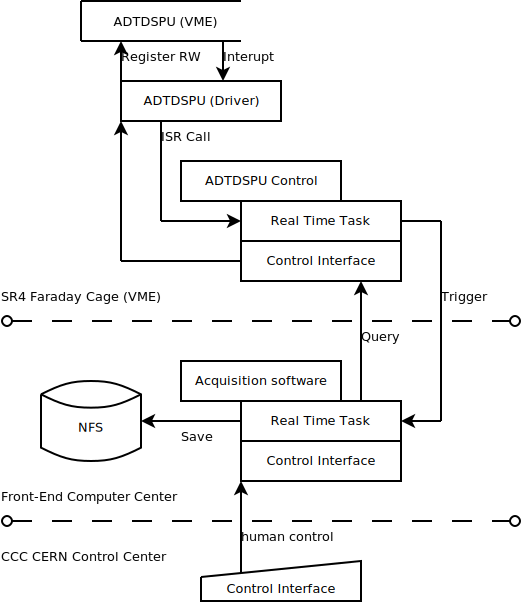
\includegraphics[scale=0.3]{ImplementedSoftFesa.pdf}
\end{figure}

In the final version the software will be merged in single executable that should run on the \gls{GPU}-enabled machine. This solution has been put into place because the present hardware is still in development and there is no way of acquiring the full 2880 bunches of the machine, the hardware is receiving the acquisition data but the \gls{VME} is not fast enough to transfer it to the \gls{CPU}.

	\subsection{ADTDSPU control software}

	The first layer that was needed is a driver that can control the \gls{VME} card and forward the interrupts. This is using standard driver framework from the \gls{CO} group at \gls{CERN}.

	Then the normal \gls{FESA} environment is used to develop a higher level software to control the card. This particular card need real time task to react to interrupt coming from the hardware to inform when new acquisition is ready to be read.

	\subsection{Acquisition software}

	The acquisition software was used to check that the idea of getting the tune out of the DSPU card was doable and being able to log the acquisition to file to be checked and processed separately.

	It uses \gls{CMW}, a library used at \gls{CERN} to communicate between different layers of the accelerators control software, to connect to the the ADTDPSU control software and get the data when they are published (at interrupt time).

	It is then able to compute the acquisition \gls{FFT} using \gls{FFTW} and display it to the operators in the \gls{CCC} where all the eight accelerators of \gls{CERN} are controlled. On the interface you can decide witch type of graph you want to see and also enable saving the data into files to be processed by the data analysis software.

	\subsection{Data analysis software}



	\begin{figure}[H]
	\caption{Time flow with different implementations and with 3000 bunches of 
	2048 points each.}
	\centering
	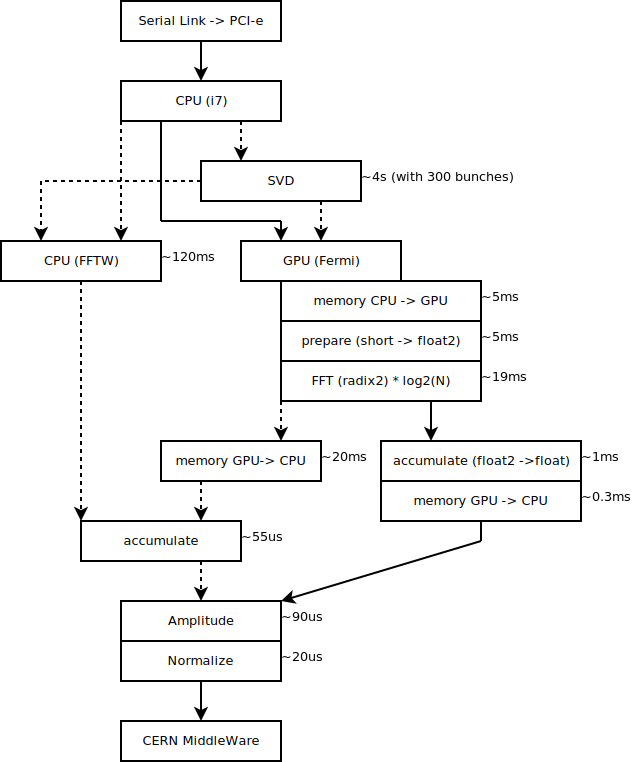
\includegraphics[scale=0.3]{PC-flow.pdf}
	\end{figure}

\section{Notch filter}

Just used to cut the low frequencies this doesn't change anything on the high frequencies and was just used to allow a better imaging on the spectrogram, it won't be used in the final version (quite slow because of sequential).

\section{FFT}

Some words about FFTs.

   \subsection{FFTW}

   Some words that explain what is FFTW and why is was chosen as a reference

   \subsection{FFT with OpenCL on GPU}

   Some words on the implementation used for calculating FFT on OpenCL reference to the image of the spectrogram.

   \subsection{FFT with OpenCL on CPU}

   Some words on the fact that you can run the code on the CPU as well and then reference on the figure.

   Also talk about the fact that there is less noise in the OpenCL CPU version than the OpenCL GPU version.

\section{Amplitude}

Amplitude calculation formula, explain the figures tell why it has to be done before accumulation and show this is very fast reference to the table of perf.

\section{SVD}

Problem is not directly solvable with the number of bunch observed cite H{\"o}fle and Rama need a lot more bunches to make a good smooth\cite{calaga06}. 

Talk about the performances issues and cite the paper on SVD on GPU as a future implementation (could go to discussion?)\cite{Lahabar09}

\section{Performances}

Calculation made by accumulation to simulate the number of bunches that could be present in the final version (2880).

   \subsection{Pipelining}

	Pipelining was tested and used in the process and it was possible to win around 15\% in performances around it.

   \subsection{Memory}

	Copy of memory from and to the GPU discution.

   \subsection{Time}

	Add table with time performances and discution.

	\begin{table}[H]
		\caption{Speed for 3000 batch of 2048 points}
		\begin{tabular}{|l|lrrcr|}
			\hline
				Device & Type & Threads & Speed [GHz] & pipeline & Time [ms] \\
			\hline
			\hline
				Xeon X5650 & FFTW & 12 & 2.67 & N/A & 291 \\
				Xeon X5650 & OpenCL & 12 & 2.67 & enable & 284 \\
				Xeon X5650 & OpenCL & 12 & 2.67 & disable & 288 \\
			\hline
				i7-3720QM & FFTW & 8 & 2.6 & N/A & 310 \\
				i7-3720QM & OpenCL & 8 & 2.6 & enable & 272 \\
				i7-3720QM & OpenCL & 8 & 2.6 & disable & 273 \\
			\hline
			\hline
				Tesla M2090 & OpenCL & 512 & 1.3 & enable & 35 \\
				Tesla M2090 & OpenCL & 512 & 1.3 & disable & 37 \\
			\hline
				GeForce 650M & OpenCL & 384 & 0.9 & enable & 355 \\
				GeForce 650M & OpenCL & 384 & 0.9 & disable & 365 \\
			\hline
		\end{tabular}
	\end{table}

\section{Spectrogram}

Some word definition of Spectrogram. Display some spectrogram.

\begin{figure}[H]
	\caption{Spectrogram with ADT off on the 16 October 2012 on vertical beam 1 during squeeze and collision}
	\centering
	\includegraphics[scale=0.3]{md-121016-vb1-m1-6bunches-10acc-1359-1425-collision.pdf}
\end{figure}